\documentclass[12pt]{article}
 
\usepackage[margin=1in]{geometry} 
\usepackage{amsmath,amsthm,amssymb}
\usepackage{graphicx}
\usepackage{float}
\usepackage{tikz}
\usetikzlibrary{arrows,shapes,trees} % loads some tikz extensions
 
\begin{document}
 
\title{Homework 5}
\author{Josh Klontz
CSE 802}
 
\maketitle

\begin{enumerate}
\item \subitem{8.}
\begin{enumerate}
\item \textbf{Show that the Bayes rate for the one-dimensional case where $P(w_i)=1/c$ and ... is $P^* = r$.}
\begin{equation}
\begin{split}
p(x) &= c\int p(x|w_i)P(w_i) dx \\
       &= c((\frac{cr}{c-1}) + (1 - \frac{cr}{c-1}))(1/c) \\
       &=1 \\
P^* &= \int min(1-P(w_i|x)) dx \\
      &= \int min(1-p(x|w_i)P(w_i)/p(x)) dx \\
      &= \int min \left(1-\left\{ \begin{array}{rl} 1 & 0\leq x \leq \frac{cr}{c-1} \\ 1 & i \leq x \leq i+1-\frac{cr}{c-1} \\ 0 & \text{elsewhere} \end{array} \right. \cdot 1/c \right) dx \\
      &= \int_0^\frac{cr}{c-1}1-\frac{1}{c}dx~~\text{(The only region where the error rate isn't zero.)} \\
      &= \frac{cr}{c-1}(1-\frac{1}{c}) \\
      &= \frac{cr}{c-1} - \frac{r}{c-1} \\
      &= \frac{cr-r}{c-1} \\
      &= r\frac{c-1}{c-1} \\
      &= r \\
      & \qed
\end{split}
\end{equation}
\item \textbf{Show that for this case the nearest-neighbor rate is $P=P^*$}
\begin{equation}
\begin{split}
P &= \int \left[1-\sum_{i=1}^c P^2(w_i|x) \right]p(x)dx \\
   &= \int \left[1-\sum_{i=1}^c (p(x|w_i)P(w_i)/p(x))^2 \right]p(x)dx \\
   &= \int 1-c \left( \left\{ \begin{array}{rl} 1/c^2 & 0\leq x \leq \frac{cr}{c-1} \\ 1/c^2 & i \leq x \leq i+1-\frac{cr}{c-1} \\ 0 & \text{elsewhere} \end{array} \right. \right)^2 dx \\
   &= \int 1- \left\{ \begin{array}{rl} 1/c & 0\leq x \leq \frac{cr}{c-1} \\ 1/c & i \leq x \leq i+1-\frac{cr}{c-1} \\ 0 & \text{elsewhere} \end{array} \right. dx \\
   &= \int_0^\frac{cr}{c-1}1-1/c~dx~~\text{As $n \to \infty$ this is the only term with non-zero error.} \\
   &= ...~\text{Same algebraic simplificaiton as (a)} \\
   &=r \\
   &=P^* \\
   & \qed
\end{split}
\end{equation}
\subitem{9.}
\begin{equation}
\begin{split}
m_1 &= [5 -4] \\
m_2 &= [3.33 6.67] \\
m_3 &= [2.33 2] \\
\end{split}
\end{equation}
\newpage
\begin{enumerate}
\item \textbf{Plot the decision boundary for $w_1$ and $w_2$.}
\begin{figure}[H]
\centering
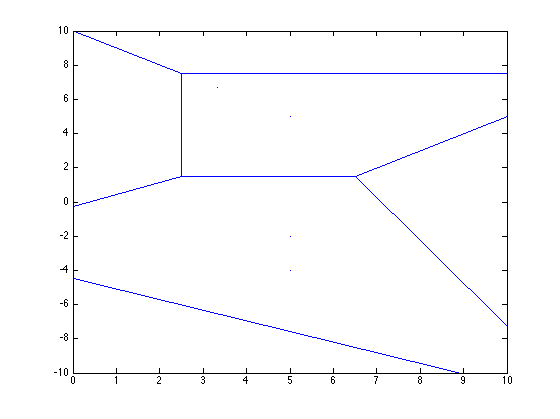
\includegraphics[width=5in]{12.png}
\end{figure}
\item \textbf{Plot the decision boundary for $w_1$ and $w_3$.}
\begin{figure}[H]
\centering
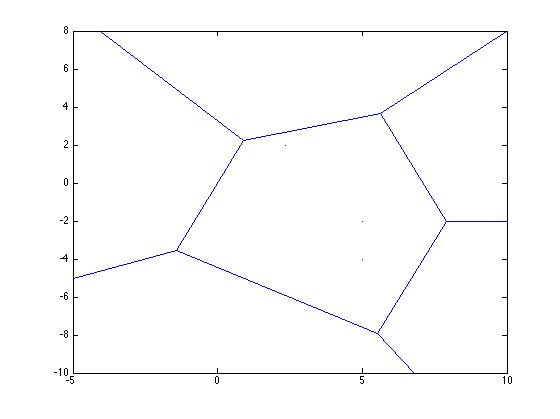
\includegraphics[width=5in]{13.png}
\end{figure}
\newpage
\item \textbf{Plot the decision boundary for $w_2$ and $w_3$.}
\begin{figure}[H]
\centering
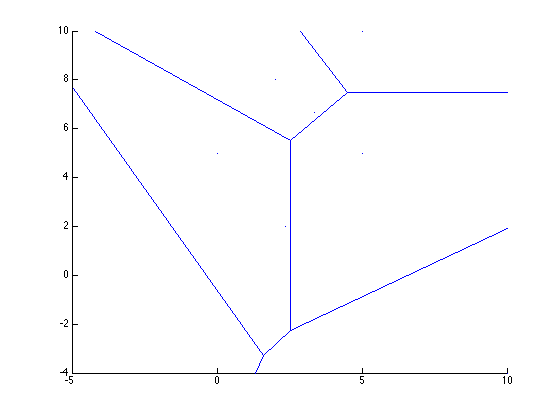
\includegraphics[width=5in]{23.png}
\end{figure}
\item \textbf{Plot the decision boundary for $w_1$, $w_2$, and $w_3$.}
\begin{figure}[H]
\centering
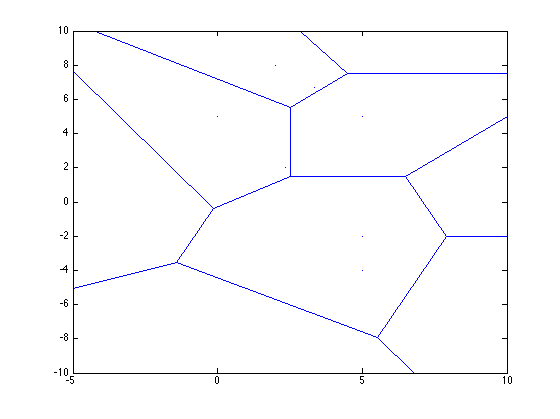
\includegraphics[width=5in]{123.png}
\end{figure}
\end{enumerate}
\end{enumerate}
\end{enumerate}
\end{document}
